%!TEX root = ../thesis.tex
%%%%%%%%%%%%%%%%%%%%%%%%%%%%%%%%%%%%%%%%%%%%%%%%%%%%%%%%%%%%%%%%%%%%%%%
%
% Implementation
%
%%%%%%%%%%%%%%%%%%%%%%%%%%%%%%%%%%%%%%%%%%%%%%%%%%%%%%%%%%%%%%%%%%%%%%%
\chapter{Implementation}%
\chaptermark{Implementation}%
\label{chapter:implementation}

\section{Technologies} 

\begin{itemize}
  \item NextJS
  \item Ant Design
  \item AWS DynamoDB
  \item AWS S3
  \item AWS Lambda functions
  \item AWS Cognito
  \item AWS AppSync
  \item GraphQL
\end{itemize}

\section{Tools} 

\begin{itemize}
  \item Visual Studio
  \item Amazon console
  \item Postman
  \item AWS Amplify
\end{itemize}

\clearpage

\section{Code Snippets} 

\begin{figure}[!hb]
\centering
\caption[Delete Comments after deleting Recipe]{Delete Comments after deleting Recipe}%
\label{fig:delete_comments}
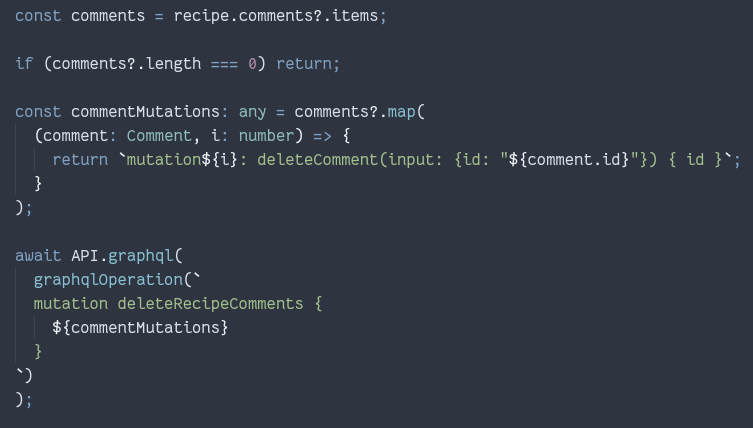
\includegraphics[width=\linewidth,height=\textheight,keepaspectratio]{img/delete_comments}
\end{figure} 

\begin{figure}[!hb]
\centering
\caption[Recipe Pagination]{Recipe Pagination}%
\label{fig:recipe_pagination}
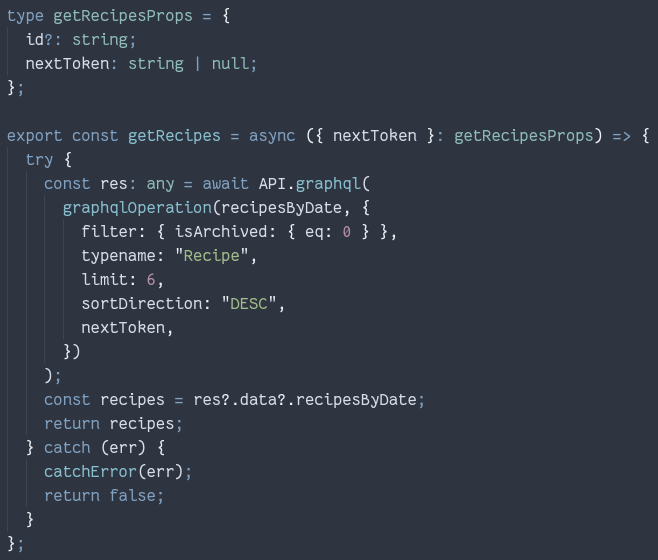
\includegraphics[width=\linewidth,height=\textheight,keepaspectratio]{img/recipe_pagination}
\end{figure} 

\clearpage

\section{NextJS File Structure} 

\begin{longtable}{p{5cm}|p{5cm}}
\caption[NextJS File Structure]{NextJS File Structure} % 
\label{tab:r1_r2_of_45} \\ 
Directory/File & \column{Description} \\ \hline
|-- theveganmanna &
\row{\linewidth}Root folder \\ \hline
%amplify%
\hspace{0.45cm}|-- amplify &
\row{\linewidth}Amplify resource files \\ \hline
%node_modules%
\hspace{0.45cm}|-- {node\_modules} &
\row{\linewidth}Dependent modules \\ \hline
%public%
\hspace{0.45cm}|-- public &
\row{\linewidth}Public assets \\ \hline
%src%
\hspace{0.45cm}|-- src &
\row{\linewidth}Main application folder \\ \hline
%api%
\hspace{0.90cm}|-- api &
\row{\linewidth}API files \\ \hline
%components%
\hspace{0.90cm}|-- component &
\row{\linewidth}Component files \\ \hline
%contexts%
\hspace{0.90cm}|-- contexts &
\row{\linewidth}React Contexts \\ \hline
%graphql%
\hspace{0.90cm}|-- graphql &
\row{\linewidth}GraphQL files \\ \hline
%graphql%
\hspace{1.35cm}|-- mutations.js &
\row{\linewidth} \\ \hline
%graphql%
\hspace{1.35cm}|-- queries.js &
\row{\linewidth} \\ \hline
%graphql%
\hspace{1.35cm}|-- subscriptions.js &
\row{\linewidth} \\ \hline
%hooks%
\hspace{0.90cm}|-- hooks &
\row{\linewidth}React Hooks \\ \hline
%interfaces%
\hspace{0.90cm}|-- interfaces &
\row{\linewidth}TypeScript Interfaces \\ \hline
%layouts%
\hspace{0.90cm}|-- layouts &
\row{\linewidth}Layout components \\ \hline
%pages%
\hspace{0.90cm}|-- pages &
\row{\linewidth}NextJS pages \\ \hline
%styles%
\hspace{0.90cm}|-- styles &
\row{\linewidth}Style files \\ \hline
%aws-exports.js%
\hspace{0.90cm}|-- aws-exports.js &
\row{\linewidth}Amplify config \\ \hline
%tests%
\hspace{0.45cm}|-- tests &
\row{\linewidth}Jest test files \\ \hline
%.babelrc%
\hspace{0.45cm}|-- .babelrc &
\row{\linewidth}Babel config \\ \hline
%graphqlconfig.yml%
\hspace{0.45cm}|-- graphqlconfig.yml &
\row{\linewidth}GraphQL config \\ \hline
%jest.config.js%
\hspace{0.45cm}|-- jest.config.js &
\row{\linewidth}Jest config \\ \hline
%next.config.js%
\hspace{0.45cm}|-- next.config.js &
\row{\linewidth}Custom webpack config \\ \hline
%package.json%
\hspace{0.45cm}|-- package.json &
\row{\linewidth}Requirements of application \\ \hline
%tsconfig.json%
\hspace{0.45cm}|-- tsconfig.json &
\row{\linewidth}TypeScript config \\ \hline
%yarn.lock%
\hspace{0.45cm}|-- yarn.lock &
\row{\linewidth}Lock file \\ 
\end{longtable}


